\documentclass[french]{report}
\usepackage[utf8]{inputenc}
\usepackage[T1]{fontenc}
\usepackage{babel}
\usepackage[autolanguage]{numprint}
\usepackage[backend=bibtex]{biblatex}
\usepackage{csquotes}
\addbibresource{bibrapport.bib}
\usepackage{graphicx}
\usepackage{wrapfig}
\usepackage{lipsum}
\usepackage{float} 
\usepackage{multirow}

\begin{document}
\begin{center}
	\LARGE \textbf{Rapport}
\end{center}
\textit{Sujet:} segmentation d'images cytologiques basée sur l'apprentissage profond\\
\textit{Auteurs:} Amin KHOUANI, Mostafa EL HABIB DAHO et Med Amine CHIKH \\
\textit{Présenté par:} Ousmane Issa.
\section*{Introduction}
La cytologie (étude des cellules isolées et leurs morphologies) faite manuellement passe par plusieurs étapes couteuses (De la culture jusqu'à l'observation microscopique), elle permet le diagnostique de maladies. La segmentation, la détection et le comptage précis des cellules à partir d'images cytologiques par des techniques d'apprentissage automatique s'avère utile pour diminuer le coût et facilement rapidement le diagnostic de certaines maladies comme le cancer. L'apprentissage profond a donné de meilleurs résultat sur la vision artificielle dans ces dernières années \cite{im1, rcnn}, il est donc un meilleur choix pour remplacer l'observation microscopique en tant qu'estimateur.

Dans cet article, les auteurs proposent de faire une adaptation de l'architecture mask RCNN qui a été proposé dans \cite{rcnn} sur des données (images) médicales de l'hôpital universitaire de Tlemcen. Ils ont prit le 75\% de la base originale sur lequel ils font modification pour augmenter la taille de leur base d'apprentissage et donne plus de chance au modèle de détecter certaines perturbations qu'on peut avoir lors de l'acquisition de l'image. mask RCNN est une amélioration de RCNN qui est un modèle de la famille de réseaux de neurones convolutifs. Ils permettent la segmentation des images en retournant des régions (des coordonnées) et leurs significations (étiquètes).   
\section*{Résultats}
Quatre configurations ont été définies fig.{\ref{comb}}, et ces configurations sont basées sur la taille des images fusionnées ou pas avec les transformations faites sur les données pour l'augmentation de la base d'apprentissage. 

\begin{figure}[H]
	\centering
	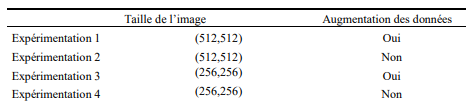
\includegraphics{images/rapport_1.PNG}
	\caption{Combinaison de configuration des modèles}
	\label{comb}
\end{figure} 

Ils mentionnent avoir obtenu  98,18\% de précision et obtenir une erreur minimale de 0.8\% d'erreurs sur la classification des cellules .
\begin{figure}[H]
	\centering
	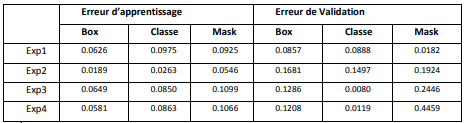
\includegraphics{images/rapport_2.PNG}
	\caption{Résultats obtenus}
	\label{comb}
\end{figure} 

\section*{Remarques}
Positivement, c'est intéressant de faire la transformation de données non seulement pour l'augmentation de la base d'apprentissage qui est un point crucial pour l'apprentissage profond mais également pour combler certaines perturbations d'acquisitions de données.\\

Tout d'abord ils mentionnent au début de l'article (résumé) d'avoir proposé un modèle pour la segmentation des images cytologiques et après dans l'article ils mentionnent encore d'avoir adapté le modèle à leurs données et aux transformation faites pour l'augmentation sans mentionner comment ils l'ont adapté. Aucune explications propres a eux de l'architecture (mask RCNN: fonction objective, algorithme d'optimisation, ...) qu'ils utilisent ou même de la famille de l'architecture n'a été fournie ce qui fait croire que le modèle lui même n'a pas été maitrisé. 

Ils n'ont mentionné aucun travail concernant la segmentions des images cytologiques pendant qu'il existe beaucoup de méthodes et modèles qui essaient de minimiser l'erreur d'estimation comme \cite{ref1, ref2} ..., donc aucun point de comparaison n'a été faite. Encore ils n'ont mentionné aucun dépôt de leur code pour une évaluation et point de comparaison.  

\section*{Conclusion}
Dans cet article, les auteurs ont essayé de minimiser l'erreur de prédiction de la segmentation des images cytologiques pour aider aux diagnostiques de certaines maladies. Des résultat ont été obtenu mais nous ne possédons aucun moyen de validation des résultats (pas de code). Aucun état de l'art  et point de comparaison n'ont été fourni. \\

\hfill score: weak accept

\printbibliography

\end{document}